

\newcommand{\gooresetup}[3]{%
	\begin{tabular}{ll}
		\toprule
		Ratio & #1 \\
		Rounds & #2 \\
		Number of players & #3 \\
		\bottomrule
	\end{tabular}}
	



\chapter{Results}
\label{ch:results}

Here we present a representative subset of the obtained results.
We provide graphs to visualise how different parameters influence the results.
We first present results for the multi-armed bandit, followed by the results for the Goore game.

Parameter values are likely to interact and impact the end result in different ways, and it may be difficult to capture these interactions directly.
By fixing all but one parameter and testing for a range of values for this parameter, we capture different aspects of how the optimal observation noise changes.

\section{Multiarmed Bandit}
\begin{figure}[hbtp]
    \hspace*{-2.5cm}
    \begin{minipage}[c]{0.39\textwidth}
        \begin{gnuplot}[terminal=epslatex,terminaloptions=color solid]
            set style data dots
            set grid
            set nokey
            set xlabel "Arms" rotate
            set ylabel "Rounds" rotate
            set zlabel "Observation noise" rotate
            set log xy
            set xyplane 0
            set xtics 2
            set xrange [2:64]
            set yrange [10:1000]
            set zrange [0:0.3]
            set palette model CMY rgbformulae 7,5,15
            set pm3d at s hidden3d 100 
            set style line 100 lt -1 lw 2
    splot "../data/bandit/good-5.0,0.5\_bad-4.0,0.5\_est-0.0,50.0\_num-(64,1.0,1.0)\_rounds-1000\_algo-UCB1.data" using 5:6:7
    \end{gnuplot}
%    % GNUPLOT: LaTeX picture with Postscript
\begingroup
  \makeatletter
  \providecommand\color[2][]{%
    \GenericError{(gnuplot) \space\space\space\@spaces}{%
      Package color not loaded in conjunction with
      terminal option `colourtext'%
    }{See the gnuplot documentation for explanation.%
    }{Either use 'blacktext' in gnuplot or load the package
      color.sty in LaTeX.}%
    \renewcommand\color[2][]{}%
  }%
  \providecommand\includegraphics[2][]{%
    \GenericError{(gnuplot) \space\space\space\@spaces}{%
      Package graphicx or graphics not loaded%
    }{See the gnuplot documentation for explanation.%
    }{The gnuplot epslatex terminal needs graphicx.sty or graphics.sty.}%
    \renewcommand\includegraphics[2][]{}%
  }%
  \providecommand\rotatebox[2]{#2}%
  \@ifundefined{ifGPcolor}{%
    \newif\ifGPcolor
    \GPcolortrue
  }{}%
  \@ifundefined{ifGPblacktext}{%
    \newif\ifGPblacktext
    \GPblacktexttrue
  }{}%
  % define a \g@addto@macro without @ in the name:
  \let\gplgaddtomacro\g@addto@macro
  % define empty templates for all commands taking text:
  \gdef\gplbacktext{}%
  \gdef\gplfronttext{}%
  \makeatother
  \ifGPblacktext
    % no textcolor at all
    \def\colorrgb#1{}%
    \def\colorgray#1{}%
  \else
    % gray or color?
    \ifGPcolor
      \def\colorrgb#1{\color[rgb]{#1}}%
      \def\colorgray#1{\color[gray]{#1}}%
      \expandafter\def\csname LTw\endcsname{\color{white}}%
      \expandafter\def\csname LTb\endcsname{\color{black}}%
      \expandafter\def\csname LTa\endcsname{\color{black}}%
      \expandafter\def\csname LT0\endcsname{\color[rgb]{1,0,0}}%
      \expandafter\def\csname LT1\endcsname{\color[rgb]{0,1,0}}%
      \expandafter\def\csname LT2\endcsname{\color[rgb]{0,0,1}}%
      \expandafter\def\csname LT3\endcsname{\color[rgb]{1,0,1}}%
      \expandafter\def\csname LT4\endcsname{\color[rgb]{0,1,1}}%
      \expandafter\def\csname LT5\endcsname{\color[rgb]{1,1,0}}%
      \expandafter\def\csname LT6\endcsname{\color[rgb]{0,0,0}}%
      \expandafter\def\csname LT7\endcsname{\color[rgb]{1,0.3,0}}%
      \expandafter\def\csname LT8\endcsname{\color[rgb]{0.5,0.5,0.5}}%
    \else
      % gray
      \def\colorrgb#1{\color{black}}%
      \def\colorgray#1{\color[gray]{#1}}%
      \expandafter\def\csname LTw\endcsname{\color{white}}%
      \expandafter\def\csname LTb\endcsname{\color{black}}%
      \expandafter\def\csname LTa\endcsname{\color{black}}%
      \expandafter\def\csname LT0\endcsname{\color{black}}%
      \expandafter\def\csname LT1\endcsname{\color{black}}%
      \expandafter\def\csname LT2\endcsname{\color{black}}%
      \expandafter\def\csname LT3\endcsname{\color{black}}%
      \expandafter\def\csname LT4\endcsname{\color{black}}%
      \expandafter\def\csname LT5\endcsname{\color{black}}%
      \expandafter\def\csname LT6\endcsname{\color{black}}%
      \expandafter\def\csname LT7\endcsname{\color{black}}%
      \expandafter\def\csname LT8\endcsname{\color{black}}%
    \fi
  \fi
  \setlength{\unitlength}{0.0500bp}%
  \begin{picture}(7200.00,5040.00)%
    \gplgaddtomacro\gplbacktext{%
      \csname LTb\endcsname%
      \put(942,1289){\makebox(0,0){\strut{} 2}}%
      \csname LTb\endcsname%
      \put(1590,1170){\makebox(0,0){\strut{} 4}}%
      \csname LTb\endcsname%
      \put(2238,1051){\makebox(0,0){\strut{} 8}}%
      \csname LTb\endcsname%
      \put(2886,933){\makebox(0,0){\strut{} 16}}%
      \csname LTb\endcsname%
      \put(3533,814){\makebox(0,0){\strut{} 32}}%
      \csname LTb\endcsname%
      \put(4180,695){\makebox(0,0){\strut{} 64}}%
      \csname LTb\endcsname%
      \put(4398,755){\makebox(0,0){\strut{} 10}}%
      \csname LTb\endcsname%
      \put(5333,1270){\makebox(0,0){\strut{} 100}}%
      \csname LTb\endcsname%
      \put(6268,1784){\makebox(0,0){\strut{} 1000}}%
      \put(920,1384){\makebox(0,0)[r]{\strut{} 0}}%
      \put(920,1727){\makebox(0,0)[r]{\strut{} 0.05}}%
      \put(920,2070){\makebox(0,0)[r]{\strut{} 0.1}}%
      \put(920,2413){\makebox(0,0)[r]{\strut{} 0.15}}%
      \put(920,2755){\makebox(0,0)[r]{\strut{} 0.2}}%
      \put(920,3098){\makebox(0,0)[r]{\strut{} 0.25}}%
      \put(920,3441){\makebox(0,0)[r]{\strut{} 0.3}}%
      \put(236,2562){\rotatebox{-270}{\makebox(0,0){\strut{}Observation noise}}}%
    }%
    \gplgaddtomacro\gplfronttext{%
      \csname LTb\endcsname%
      \put(2198,830){\makebox(0,0){\strut{}Arms}}%
      \put(6029,1156){\makebox(0,0){\strut{}Rounds}}%
      \put(236,2562){\rotatebox{-270}{\makebox(0,0){\strut{}Observation noise}}}%
      \put(6641,2280){\makebox(0,0)[l]{\strut{} 0}}%
      \put(6641,2535){\makebox(0,0)[l]{\strut{} 0.05}}%
      \put(6641,2790){\makebox(0,0)[l]{\strut{} 0.1}}%
      \put(6641,3045){\makebox(0,0)[l]{\strut{} 0.15}}%
      \put(6641,3300){\makebox(0,0)[l]{\strut{} 0.2}}%
      \put(6641,3555){\makebox(0,0)[l]{\strut{} 0.25}}%
      \put(6641,3810){\makebox(0,0)[l]{\strut{} 0.3}}%
    }%
    \gplbacktext
    \put(0,0){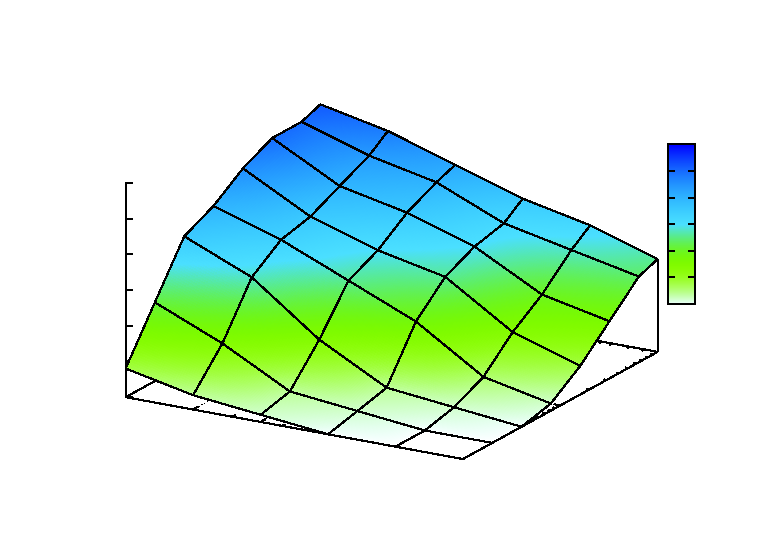
\includegraphics{armsplot}}%
    \gplfronttext
  \end{picture}%
\endgroup

    \end{minipage}
    \hspace*{7.5cm}
    \begin{minipage}[c]{0.49\textwidth}
    \banditsetup{5.0}{4.0}{0.5}{2 -- 64}{10 -- 1000}
    \end{minipage}
    \caption{Best observation noise varying with the number of arms. Note the logarithmic scales on the \emph{Arms} and \emph{Rounds} axes.}
\label{fig:numarms}
\end{figure}

As the horizon is extended, the overall trend is for \obstar{} to increase.
This can quite simply be explained if we think of the observation noise as regulating the rate of exploration.
When more time is available, more of it should be allocated for exploration in order to make it more certain that the best arm is discovered and exploited.

We first look at the case where the number of arms is changed, from the simplest case with 2 arms to a comparatively hard problem with 64 arms.
This corresponds directly to increasing the complexity of the environment, and so we get the first indication that observation noise can be used as a complexity measure: a low \obstar{} indicates a complex environment, and as the best observation noise increases the environment gradually becomes simpler.
Intuitively, in a complex environment we need to limit exploration by being more greedy in our choice of arms, as most of the arms pulled for exploration’s sake will be suboptimal.
This effect is nicely illustrated in figure~\ref{fig:numarms}, where we have varied the number of arms available to the player in a specific setting.
We see that \obstar{} exhibits approximately logarithmic growth as the number of rounds increase, and exponential decay as the number of arms increase.

\begin{figure}[htbp]
    \hspace*{-2.5cm}
    \begin{minipage}[c]{0.39\textwidth}
    \begin{gnuplot}[terminal=epslatex,terminaloptions=color solid]
    set grid
    set nokey
    set style data dots
    set pm3d at s hidden3d 100
    set style line 100 lt -1 lw 2
    set ylabel "Bad arm mean" rotate
    set xlabel "Rounds" rotate
    set zlabel "Observation noise" rotate
    set xyplane 0
    set ytics 3,0.5
    set xtics 100,100
    set xrange [100:1000]
    set yrange [3:4.5]
    set view 40,36
    set palette model CMY rgbformulae 7,5,15
    splot "../data/bandit/good-5.0,0.5\_bad-(0.5,4.5,0.5),0.5\_est-10.0,2.0\_num-5\_rounds-1000\_algo-UCB1.data" using 6:3:7
#    set style data lines
#    set xlabel "Bad arm mean" rotate
#    set ylabel "Observation noise" rotate
#    set xtics 0.5
#    set xrange [3.0:4.5]
#    plot "../data/bandit/good-5.0,0.5\_bad-(0.5,4.5,0.5),0.5\_est-10.0,2.0\_num-5\_rounds-1000\_algo-UCB1.data" using (column(6)==1000?column(3):NaN):7
    \end{gnuplot}
    \end{minipage}
    \hspace*{7.5cm}
    \begin{minipage}[c]{0.49\textwidth}
    \banditsetup{5.0}{0.5 -- 4.5}{0.5}{5}{1000}
    \end{minipage}
    \caption{Best observation noise varying with the mean on the suboptimal arms.}{As the mean is lowered past 3 or so changing observation noise stops having an effect, so these numbers are excluded from this figure.}
\label{fig:badmean}
\end{figure}

Next we modify problem difficulty by changing the expected value of the bad arms.
Again we see that as complexity is decreased by narrowing the gap between the expected values -- lessening the penalty of choosing suboptimal arms -- \obstar{} also decreases.
This effect is illustrated in figure~\ref{fig:badmean}, where \obstar{} increases along with the mean of the bad arms.

\begin{figure}[htbp]
    \hspace*{-2.5cm}
    \begin{minipage}[c]{0.39\textwidth}
    \begin{gnuplot}[terminal=epslatex,terminaloptions=color solid]
    set nokey
    set pm3d
    set ylabel "Standard deviation" offset 0,-1
    set xlabel "Rounds" offset 1,-1
    set zlabel "Observation noise" rotate
    set xyplane 0
    set palette model CMY rgbformulae 7,5,15
    set view 65,312
    set xtics 200 offset -1.2,0.-0.5
    set xrange [10:1000]
    set yrange [0.1:5.1]
    set zrange [0.01:4.6]
    set ytics 0.1,1.0
    set ytics offset 0,-0.5
    splot '../data/bandit/good-5.0,(0.1,5.0,0.5)_bad-4.0,(0.1,5.0,0.5)_est-0.0,50.0_num-2_rounds-1000_algo-UCB1.data' using 6:2:7 with line lt -1 lw 2
    #splot "../data/bandit/good-6.5,(0.1,5.0,0.9)\_bad-4.0,(0.1,5.0,0.9)\_est-0.0,50.0\_num-5\_rounds-1000\_algo-UCB1.data" using 6:2:7 with line lt -1 lw 2 title ""
    \end{gnuplot}
    \end{minipage}
    \hspace*{7.5cm}
    \begin{minipage}[c]{0.49\textwidth}
    \banditsetup{5.0}{4.0}{0.1 -- 5.1}{2}{10 -- 1000}
    \end{minipage}
\caption{Varying standard deviation.}
\label{fig:gooddev}
\end{figure}

On the other hand, in figure~\ref{fig:gooddev} we see that increasing the uncertainty of rewards by increasing the variance of the best arm has the effect of increasing \obstar{}.
So the notion that smaller \obstar{} indicates a more complex environment may be too simplistic.

\begin{figure}[htbp]
    \hspace*{-2.5cm}
    \begin{minipage}[c]{0.39\textwidth}
    \begin{gnuplot}[terminal=epslatex,terminaloptions=color solid]
    set style data lines
    set grid
    set xlabel "Rounds"
    set ylabel "Instant regret"
    set log x
    set xrange [4:1000]
    plot "../data/instantrewards/good-5.0,2.0\_bad-4.0,2.0\_est-10.0,50.0\_num-2\_obnoise-0.51\_rounds-1000\_reps-100000\_algo-LTS\_kind-Instant.data" using 1:(5-column(2)) title "LTS (\\ob{} = 0.51)", \
         "../data/instantrewards/good-5.0,2.0\_bad-4.0,2.0\_num-2\_rounds-1000\_reps-100000\_algo-UCB1\_kind-Instant.data" using 1:(5-column(2)) title "UCB1"
    \end{gnuplot}
    \end{minipage}
    \hspace*{7.5cm}
    \begin{minipage}[c]{0.49\textwidth}
    \banditsetup{5.0}{4.0}{2.0}{2}{1 -- 1000}
    \end{minipage}
\caption{Instant regret for UCB1 and LTS.}
\label{fig:ucbcomp}
\end{figure}

LTS is superior to UCB1 when the optimal observation noise value is selected.
In figure~\ref{fig:ucbcomp} this is demonstrated:
Even though UCB1 performs reasonably good from the start it is rapidly overtaken by LTS.

\section{Goore Game}

The optimal value for the observation noise is found at the highest reward given to the players.
In figure \ref{fig:ex12} one can see that the optimal noise is between 1.3 and 1.4. Any higher or any lower 
observation noise will quickly lead to less reward. The drop is steeper if the observation noise is less than 1.3 compared to if the observation noise is greater than 1.4. The reason for this is that when players decide too quickly the correct ratio may not be achieved in time. In figure \ref{fig:ex8} one can see that with a greater Gaussian white noise a higher observation noise is needed to achieve the optimal reward. In addition, the optimal observation noise rises if the players are able to play Goore game for a long time. By having 
more time the players can spend more time exploring and still have plenty of time left to exploit the Goore game for reward. 

\begin{figure}[htbp]
    \hspace*{-2.5cm}
    \begin{minipage}[c]{0.39\textwidth}
    \begin{gnuplot}[terminal=epslatex,terminaloptions=color solid]
    set grid
    set xrange [0.9:1.8]
    set style data lines
    set xlabel "Observation noise"  
    set ylabel "Reward" rotate
    plot "../python/datafolder/obsdata_repetitions-10000_bandits-40_rounds-1000_ratio-0.3_noise-1.1.data" title ""
    \end{gnuplot}
    \end{minipage}
    \hspace*{7.5cm}
    \begin{minipage}[c]{0.49\textwidth}
    \gooresetup{0.3}{1 000}{40}
    \end{minipage}
\caption{Overview of observation noise}
\label{fig:ex12}
\end{figure}

\begin{figure}[htbp]
    \hspace*{-2.5cm}
    \begin{minipage}[c]{0.39\textwidth}
    \begin{gnuplot}[terminal=epslatex,terminaloptions=color solid]
    set grid
    set style data lines
    set key left
    set ylabel "Observation noise" rotate 
    set xlabel "Gaussian white noise"
    set xrange [0.1:3.9]
    plot for [m in "10 100 1000"] "../python/3ddata/new_created_data.data" using 4:($1==m."0.0"&&$2==10.0&&$3==0.2?$5:1/0) title m."0.0 Rounds"
    \end{gnuplot}
    \end{minipage}
    \hspace*{7.5cm}
    \begin{minipage}[c]{0.49\textwidth}
    \gooresetup{0.2}{In graph}{10}
    \end{minipage}
\caption{Finding the optimal observation noise.}
\label{fig:ex8}
\end{figure}

\begin{figure}[htbp]
    \hspace*{-2.5cm}
    \begin{minipage}[c]{0.39\textwidth}
    \begin{gnuplot}[terminal=epslatex,terminaloptions=color solid]
    set grid
    set style data lines
    set key left
    set ylabel "Observation noise" rotate 
    set xlabel "Gaussian white noise"
    set xrange [0.1:3.9]
    plot for [m in "2 3 4"] "../python/3ddata/new_created_data.data" using 4:($1==10000.0&&$2==10.0&&$3=="0.".m?$5:1/0) title "0.".m." Ratio"
    \end{gnuplot}
    \end{minipage}
    \hspace*{7.5cm}
    \begin{minipage}[c]{0.49\textwidth}
    \gooresetup{In graph}{10 000}{10}
    \end{minipage}
\caption{Change in ratio effects the optimal observation noise.}
\label{fig:ex9}
\end{figure}


The ratio of yes and no can also impact the optimal observation noise, where 1 is all yes and 0 is all no.
The closer the ratio gets to 0 or 1, the optimal observation noise rises as shown in figure \ref{fig:ex9}. 
As the ratio gets closer to either extreme a bad reward given to the player may not be because of this players choice but rather because of the other players choices. Meaning that the closer the ratio it is to 0 or 1 the more the players affect each other. The number of bandits do not seem to affect the optimal observation noise too much, as shown in figure \ref{fig:ex10}. The only difference is at the starting point when the Gaussian white noise is low. As the Gaussian white noise gets higher the different configuration of players converge on the same optimal observation noise.

\begin{figure}[htbp]
    \hspace*{-2.5cm}
    \begin{minipage}[c]{0.39\textwidth}
    \begin{gnuplot}[terminal=epslatex,terminaloptions=color solid]
    set grid
    set style data lines
    set key left
    set ylabel "Observation noise" rotate 
    set xlabel "Gaussian white noise"
    set xrange [0.1:3.9]
    plot for [m in "4 7 10"] "../python/3ddata/new_created_data.data" using 4:($1==10000.0&&$2==m.".0"&&$3==0.3?$5:1/0) title m." Players"
    \end{gnuplot}
    \end{minipage}
    \hspace*{7.5cm}
    \begin{minipage}[c]{0.49\textwidth}
    \gooresetup{0.3}{10 000}{In graph}
    \end{minipage}
\caption{Change in number of players.}
\label{fig:ex10}
\end{figure}

Figure \ref{fig:ex11} shows how both number of rounds and Gaussian white noise affects the optimal observation noise for the Goore game. As seen in the figure, by having more rounds and a high Gaussian white noise it is optimal to have a high observation noise. Meaning that players should spend more time exploring this very uncertian environment to find the optimal configuration of choices. Additionally if you have a low Gaussian white noise and a high amount of rounds, the optimal observation noise is  higher than if you have high Gaussian white noise and few rounds. Naturally, a high amount of Gaussian white noise causes high variance. Given high Gaussian white noise
and a short amount of time to explore the observation varies as it is hard for players to decide on the correct configuration and thus the results are generally poor.

\begin{figure}[htbp]
    \hspace*{-2.5cm}
    \begin{minipage}[c]{0.39\textwidth}
    \begin{gnuplot}[terminal=epslatex,terminaloptions=color solid]
    set grid
    set xrange [10:10000]
    set log x
    set pm3d
    set xyplane 0
    set view 60,310
    set palette model CMY rgbformulae 7,5,15
    set style data lines
    set zlabel "Observation noise" rotate 
    set ylabel "Gaussian white noise"
    set xlabel "Rounds"
    splot "../python/3ddata/new_created_data.data" every 4 using 1:4:($2==10.0&&$3==0.3?$5:1/0) with line lt -1 lw 1 title ""
    \end{gnuplot}
    \end{minipage}
    \hspace*{7.5cm}
    \begin{minipage}[c]{0.49\textwidth}
    \gooresetup{0.3}{In graph}{10}
    \end{minipage}
\caption{Overview of Rounds and Gaussian white noise}
\label{fig:ex11}
\end{figure}

